\chapter{Introduction}
\label{chapter:introduction}

The \gls{iot} has been one of the major technology trends in the last years. \gls{iot} represents a general concept for the ability of network devices to sense and collect data from the world around us, and then share that data across the Internet where it can be processed and utilized for various interesting purposes. \gls{iot} is considered a revolution in terms of communication between devices.

The ability to determinate the position of devices or people inside buildings is one of the most important features in \gls{iot} and its development goes far beyond the red dot on a map, making positioning an important field of application for \gls{iot}. 
An application scenario, where the positioning data in stores leads to significant added value, is the anonymous tracking of customers itineraries. The system can analyse the data and conclude which products are more interesting or have greater popularity. It can also suggest other products associated to the ones seen before.

\gls{ble} is a key building block for the \gls{iot}, thanks to its pervasiveness due to the mobile devices support of Bluetooth 4.0, low-power consumption and protocol optimization for low-rate transmission.
Even though beacons are very simple, they are a technological advancement because they allow for indoor positioning and subsequently indoor behaviour tracking. They create a new seamless interaction that does not consume a lot of battery.

These \gls{ble} beacons are often described as "Smart Devices" in \gls{iot}. It is possible to extract information from certain objects just by bringing our device close to it. Non-processor entity whose data can be acquired and migrated over internet falls under these category. 

\begin{comment}

The system consists of base stations, mobile stations, a processing server and a web server. The base stations are implemented with custom software installed on WiFi and Bluetooth Low Energy (BLE) enabled Raspberry Pi’s. BLE beacons from Estimote are used as mobile stations. The base stations listen for mobile stations and the processing server collects information from the base stations. The web server hosts a custom web client developed in AngularJS that fetches real-time updates from the processing server and presents relevant information to first responders or system administrators. The processing server and web server may run on the same physical machine.
To estimate the position of a mobile station, RSSI based distance estimates are induced into a trilateration algorithm on the processing server. To increase the accuracy of the position estimates, a technique to continuously calibrate the path loss exponent was implemented.
------
Even though beacons are very simple, they are a technological advancement: They allow for indoor positioning (something that GPS is not able to provide) and subsequently indoor behavior tracking. They create a new seamless interaction that does not consume a lot of battery. Due to its simplicity, beacon technology does not need to battle as many standards as other IoT applications.
-------
Bluetooth Low Energy (BLE) is a key building block for the IoT, thanks to its pervasiveness (mobile devices support Bluetooth 4.0), low-power consumption and protocol optimization for low-rate transmission. 
BlueUp supports you in your projects based on BLE devices and beacons, offering state-of-art and enterprise-grade products and solutions, tailored for your needs.
\end{comment}

\begin{comment}
-------
3.2 What are Smart Objects?

We find the mention of "Smart Objects" and "Smart Devices" quite often in general defination and description of IoT alongside network connectivity of embedded system. But what exactly are smart object?

Quote:
A Smart Object is an object that can describe its own possible interactions. 

Any object which not only has a state, which has certain data associated with a state but an object which can also determine nature of connectivity, duration of connectivity and connectivity protocol are called smart objects.

Radio Frequency Identification (RFID), Bluetooth Low Energy (BLE), and Near Field Communication (NFC)  makes it possible to use our phone as readers. We can extract information from certain objects just by tapping it or bringing our device close to it. RFID tags does not have any embedded system nor does a NFC tag has. But data can still be brought to internet by reading through a reader. These are called smart objects.  Non-processor entity whose data can be acquired and migrated over internet falls under these category. 
\end{comment}

%url{http://www.pcworld.com/article/2000276/a-brief-history-of-gps.html}

%\url{http://info.atollic.com/hs-fs/hub/460400/file-2653641781-jpg/Blog/iot.jpg}

%\url{https://www.infsoft.com/blog-en/articleid/135/internet-of-things-and-indoor-positioning#}
\section{Problem definition}
\label{section:problem}

Commercial, ludic and scientific spaces, most of the times, cannot or have difficulty in directing users to their interest. Spaces use different ways to achieve this goal, for example, stores use discounts to increase their sales of certain products. The fact that sometimes discounts go unnoticed is related to the way owners or administrators spread the information, which does not guarantee reaching efficiently the customers. It would be easier, if the customers could receive the information in a mobile phone application, at the right time and in the right situation. On the other hand, the administrators have doubts where to put the information available to the users. It would be useful, if the information about the localization of their consumers was provided to the owners or administrators. 
Therefore, arises the need for a positioning system in an indoor environment that can localize devices and transmit the information that both clients and owners want.
%
%acho que o problema não é o receberem ou não toda a informação e receberem-na no telefone ou de outra forma.  O problema é receberem-na no momento e situação certo.  É para isso que o conhecimento da posição de um cliente dentro de uma loja ajuda.  O telefone é um mero instrumento que é pratico usar pois toda a gente tem um (assume-se).
%%%%%%%%%%%%%%%%%%%%%%%%%%%%%%%%%%%%%%%%%%%%%%%%%%%%%%%%%%%%%%%%%%%%%%%%
\section{Motivation}
\label{section:motivation}
Having in mind the need for a positioning system in an indoor environment, many different solutions for achieving the user's positioning have been proposed. An interesting setting is one where Bluetooth beacons can interact with mobile phones and a processing server. The mobile phone has the hardware necessary for \gls{wi-fi} and \gls{ble} enabled. The mobile phone application listens for \gls{ble} beacons advertisements and the processing server collects information from the mobile phone. In Figure \ref{fig:motiv} a visual description of this system is given.
To estimate the position of a mobile phone, \gls{rssi} based distance estimates are induced into an algorithm on the processing server, it is possible to do this calculation in the mobile phone application if the mobile phone has sufficient capacity to do this calculus.

\begin{figure}[!htb]
	\centering
	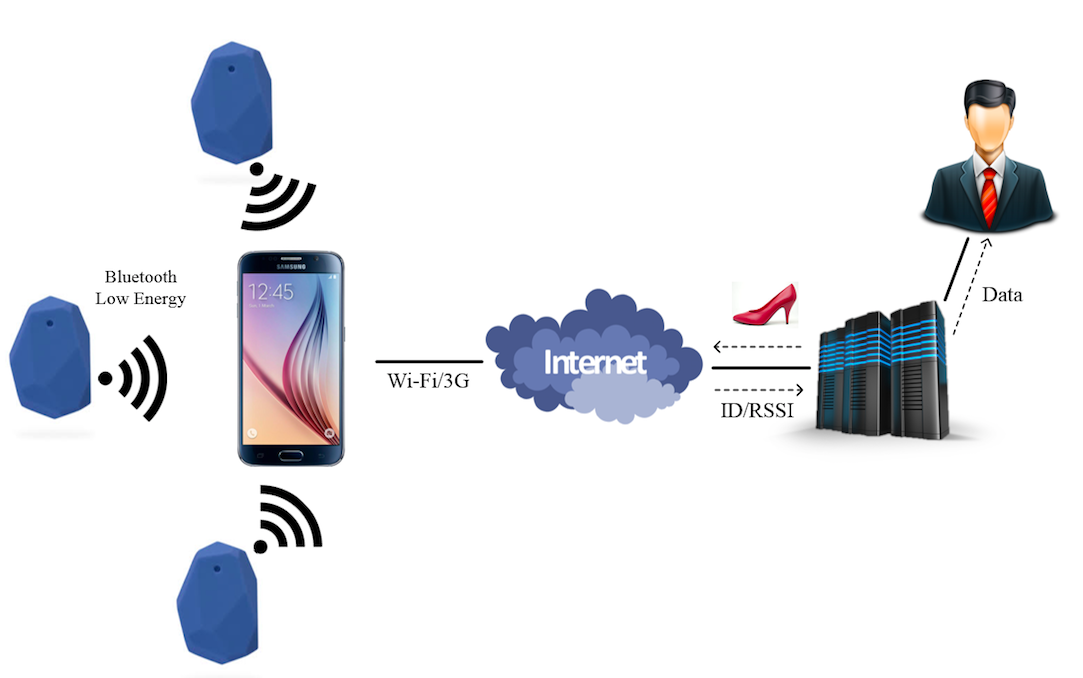
\includegraphics[width=1\textwidth]{Figures/architecture.png}
	\caption[Architecture of the positioning system]{Architecture of the positioning system.}
	\label{fig:motiv}
\end{figure} 

\begin{comment}

The idea of having access control be aware of a user’s location is an interesting concept and an ongoing research area. Many different solutions for achieving this location awareness have been proposed, for instance WiFi signal strength triangulation, radio- and ul- trasound transmitters, combinations of WiFi signals and accelerometers, etc. Issues with existing solutions include overspecialization, custom hardware requirements or active user interaction. A new method for achieving Location Aware Access Control (LAAC) should thus be simple, affordable, require no actual end-user interaction to function, and support as many modern portable devices as possible. 

A simple-to-use and reliable solution will hopefully lead to more security systems making use of location data, all while accruing relatively small costs. This is where the idea of BLE beacons comes in. Many modern portable devices supports receiving and transmitting BLE signals and the transmitters are cheap, small and energy efficient.

------------
"50 billion connected devices by 2020". Ericsson’s former \gls{ceo}, Hans Vestburg, stated it in a 2010 presentation to shareholders\footnote{https://www.ericsson.com/thecompany/press/releases/2010/04/1403231}. The next year, Dave Evans, who worked for Cisco\footnote{http://www.cisco.com}, published the same prediction in~\citep{cisco}. With this in mind, new technologies have been developed and improved to facilitate the communication between devices. Therefore, a revolution has arisen in the way positioning systems have been deployed.
\end{comment}

%http://www.ics.uci.edu/~cs237/ProjectSlidesSpring2015/15.pdf

%http://academia.stackexchange.com/questions/44784/how-to-explain-things-in-the-motivation-section-of-a-mathematical-paper-without

%\url{http://www.fiercewireless.com/wireless/ericsson-backs-away-from-expectation-50b-connected-devices-by-2020-now-sees-26b}

%\url{http://spectrum.ieee.org/tech-talk/telecom/internet/popular-internet-of-things-forecast-of-50-billion-devices-by-2020-is-outdated}
%%%%%%%%%%%%%%%%%%%%%%%%%%%%%%%%%%%%%%%%%%%%%%%%%%%%%%%%%%%%%%%%%%%%%%%%

%%%%%%%%%%%%%%%%%%%%%%%%%%%%%%%%%%%%%%%%%%%%%%%%%%%%%%%%%%%%%%%%%%%%%%%%
\section{Objectives}
\label{section:objectives}

The objective of this work consists in the elaboration of a system in an indoor environment that uses positioning methods to determine the position of users in a certain space.
A mobile phone application must be developed. This application receives location information from a set of beacons placed in an indoor environment. Based on that, it gets relevant information from a local or remote database and makes that information available to the user dynamically, as the user moves and his or hers position changes.
The accuracy of positioning obtained with \gls{ble} technology and the positioning methods is also checked.

%Isto continua telegrafico.  Nunca falas da aplicação?  Não é objectivo do trabalho também?  Que tal dizeres que o sistema consistirá numa aplicação que recebe informação de localização de um conjunto de beacons colocados num indoor environment e que com base nessa localização obtem informação relevante duma base de dados local (ou remota) e disponibiliza essa informação dinamicamente ao utilizador à medida que ele se desloca e a sua posição se altera???

%%%%%%%%%%%%%%%%%%%%%%%%%%%%%%%%%%%%%%%%%%%%%%%%%%%%%%%%%%%%%%%%%%%%%%%%
\section{Document Outline}
\label{section:outline}

This document is organized as follows:

\textbf{Chapter 2 (Background)}
provides the necessary background information and the state of the art related work;

\textbf{Chapter 3 (Design Choices)}
introduces the architecture of the positioning system, describes its components and implementation scenarios;

\textbf{Chapter 4 (Thesis Planning)}
presents a Gantt diagram and an explanation about the planning of the work that is going to be done next semester.
